\section*{Dati e risultati}

Graficando i dati misurati, si ottiene un grafico come quello in Figura \ref{fig:meas}, da cui si può gia stimare
che il punto di inversione è attorno a \SI{6}{\milli\litre}.

Poichè le incertezze sulla conduttanza sono trascurabili rispetto a quelle sul volume, abbiamo eseguito un fit preliminare
solo con le incertezze sulla conduttanza. Poi abbiamo trasferito le incertezze dal volume alla conduttanza grazie alla regressione preliminare.
Infine abbiamo svolto una nuova regressione con i valori trasferiti delle incertezze. 

\begin{SCfigure}[0.45][t]
    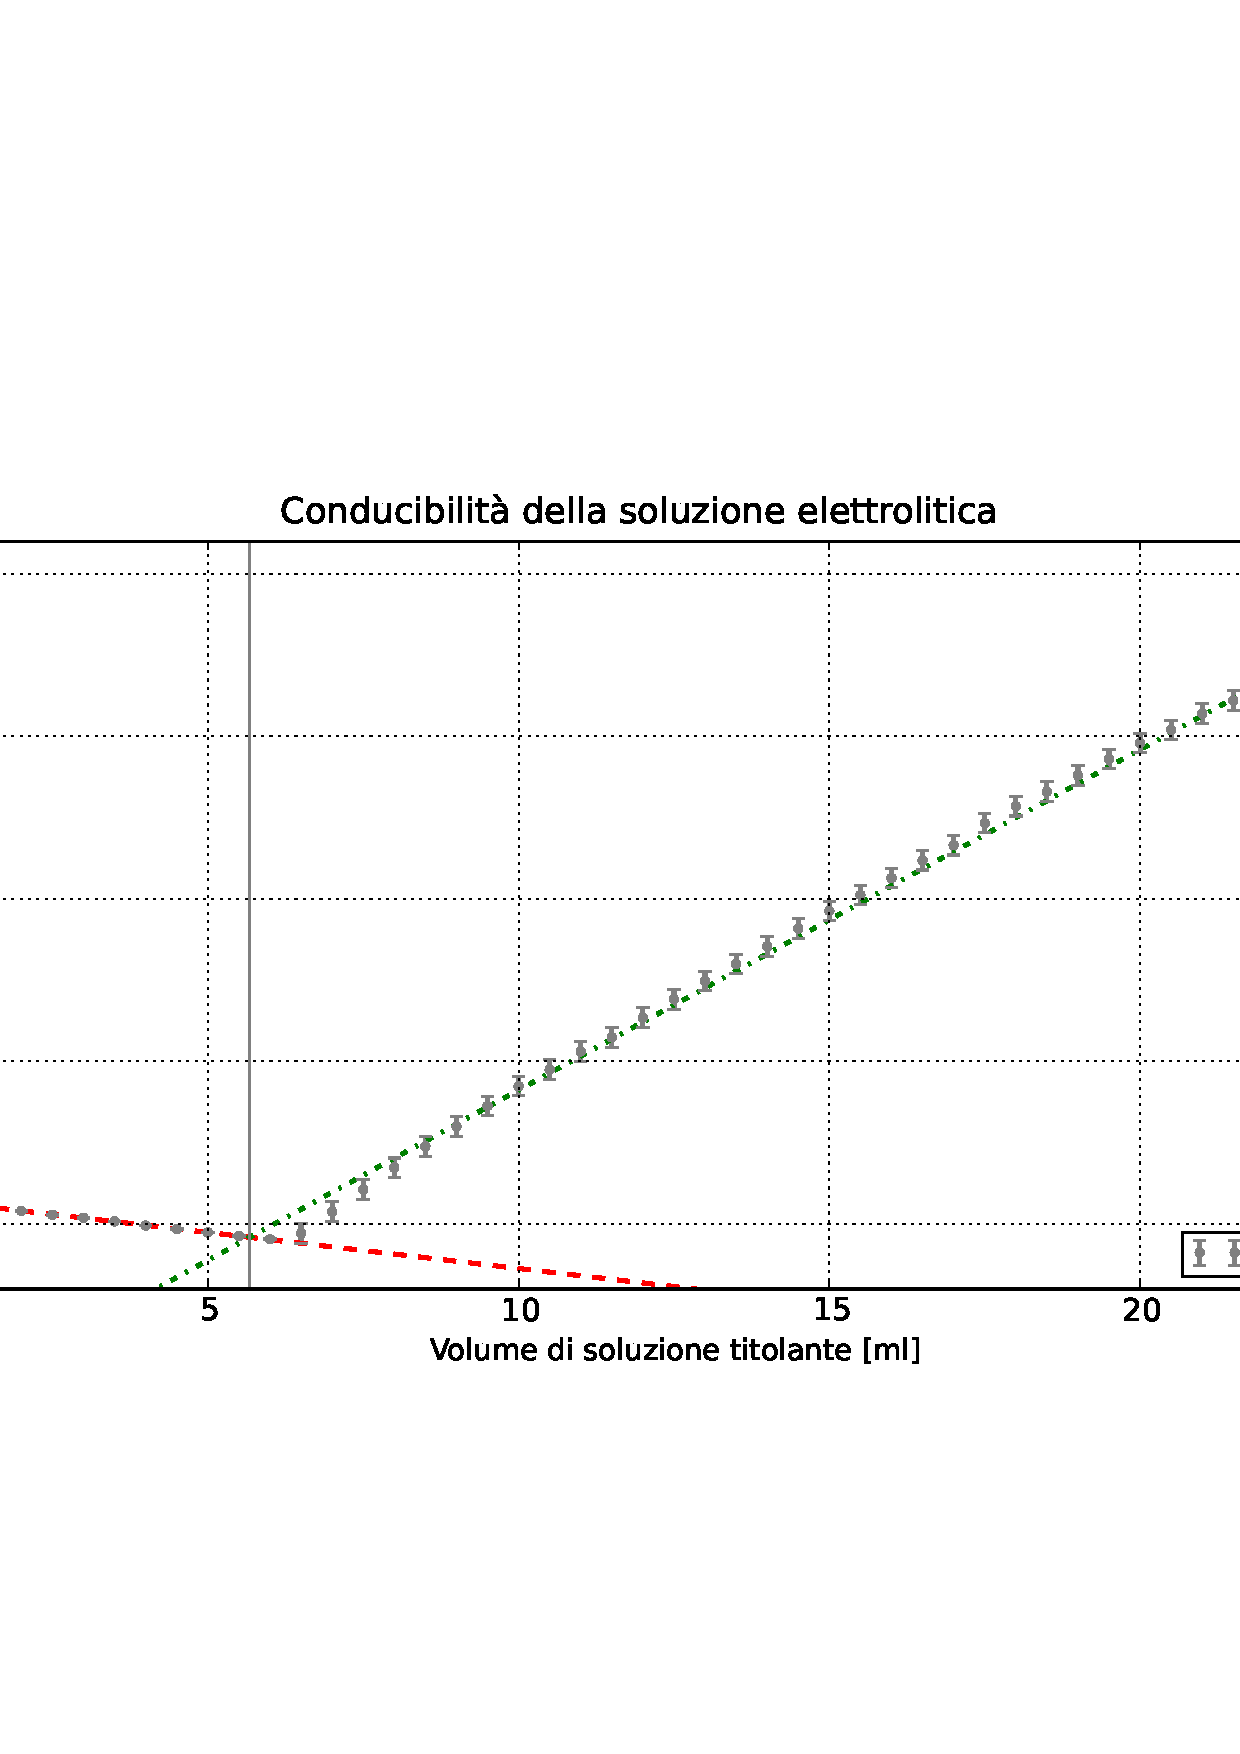
\includegraphics[scale=0.5]{Rette_von_Fitt.pdf}
    \caption{Il grafico illustra i dati  misurati, con relative incertezze, le regressioni lineari
        e il punto di intersezione tra le rette. Si vede bene che l'andamento della conducibilità
        nella serie di dati ``in salita'' non è propriamente lineare.
        Questo fatto ha causato dei problemi nel calcolo del punto di intersezione tra le rette,
        essendo la seconda retta non ben definita.
        Poichè le incertezze sono state corrette, i dati della serie
        in discesa hanno un incertezza minore di quelli della serie in salita.}
    \label{fig:meas}
\end{SCfigure}

\`E stato effettuato il test del chi quadro per verificare che la retta di fit fosse soddisfacente e che le incertezze fossero corrette.
Per la prima retta abbiamo usato i primi 13 dati; poichè una retta ha due parametri (pendenza ed intercetta),
il numero di gradi di libertà è 13 - 2 = 11. Per la retta che riguarda la salita abbiamo 38 dati e quindi la distribuzione del $\chi^2$ ha 36 gradi di libertà.
I valori attesi\footnote{L'incertezza sul valore atteso della distribuzione del chi quadro vale $\sqrt{\text{numero gradi di libertà}}$.} del $\chi^2$ erano
dunque $11 \pm 3$ e $36 \pm 6$ rispettivamente per la retta in discesa ed in salita.

I valori da noi calcolati sono stati 18 e 3657. In nessuno dei due casi il chi quadro è compatibile con il suo valore atteso.
Abbiamo quindi corretto le incertezze (le incertezze corrette sono riportate sul grafico) imponendo il valore del chi quadro
atteso. 

Le incertezze sulla conducibilità corrette sono risultate essere \SI{0.01}{\milli\siemens} per la retta in discesa e di
\SI{0.3}{\milli\siemens} per quella in salita. Il primo valore è verosimile, poiché il conduttimetro aveva la risoluzione del centesimo di mS, mentre
il secondo è abbastanza grande, sicuramente soprastimato. Questo può essere dovuto al fatto che abbiamo preso molti dati dopo il punto di inversione di tendenza,
e l'andamento è approssimativamente lineare, ma non esattamente (vedi Figura \ref{fig:meas}). Per questo motivo una retta riesce a seguire solo approssimativamente
l'andamento reale; la correzione delle incertezze non è del tutto giustificata in questo caso, anche se ci permette di salvare l'esperienza e di ottenere una stima
della concentrazione incognita. A conferma di questo fatto, si può notare che il punto di incontro tra le due rette è sottostimato: risulta minore dell'ultimo punto della serie
in discesa di dati. Ci aspettiamo quindi che dai calcoli escano valori di volume di soluzione titolante e di concentrazione sottostimati.
Per un approccio alternativo a questo problema si leggano le conclusioni.

È stato quindi rieseguito il fit con le incertezze corrette, per ottenere le incertezze corrette sui parametri delle rette.
I valori definitivi di pendenza ed intercetta sono risultati essere:

\begin{equation*}
    \text{Discesa: }
    \left\{    
    \begin{array}{l}
        m_1 = -0.222 \pm 0.001 ~ \si{\milli\siemens\per\milli\litre} \\
        q_1 = 10.849 \pm 0.005 ~ \si{\milli\siemens} \\
    \end{array}
    \right.
    \qquad
    \qquad
    \text{Salita: }
    \left\{    
        \begin{array}{l}
        m_2 = 1.05 \pm 0.01 ~ \si{\milli\siemens\per\milli\litre} \\
        q_2 = 3.65 \pm 0.15 ~ \si{\milli\siemens} \\
    \end{array}
    \right.
\end{equation*}

L'intersezione tra le due rette indica il volume di soluzione titolante versato per raggiungere
il punto di inversione, e vale:

\begin{equation*}
    p = 5.7 \pm 0.1 ~ \si{\milli\litre}
\end{equation*}

Quindi sapendo la concentrazione molare della soluzione titolante, che una mole di NaCl sostituisce una mole di \ce{AgNO3},
e che il volume iniziale della soluzione titolanda vale 100 ml si ricava facilmente la concentrazione incognita:

\begin{equation*}
    c = 0.085 \pm 0.003 ~ \text{M}
\end{equation*}

